\documentclass[11pt,]{article}
\usepackage[left=1in,top=1in,right=1in,bottom=1in]{geometry}
\newcommand*{\authorfont}{\fontfamily{phv}\selectfont}
\usepackage[]{mathpazo}


  \usepackage[T1]{fontenc}
  \usepackage[utf8]{inputenc}

\usepackage{float}
\let\origfigure\figure
\let\endorigfigure\endfigure
\renewenvironment{figure}[1][2] {
    \expandafter\origfigure\expandafter[H]
} {
    \endorigfigure
}

\usepackage{abstract}
\renewcommand{\abstractname}{}    % clear the title
\renewcommand{\absnamepos}{empty} % originally center

\renewenvironment{abstract}
 {{%
    \setlength{\leftmargin}{0mm}
    \setlength{\rightmargin}{\leftmargin}%
  }%
  \relax}
 {\endlist}

\makeatletter
\def\@maketitle{%
  \newpage
%  \null
%  \vskip 2em%
%  \begin{center}%
  \let \footnote \thanks
    {\fontsize{18}{20}\selectfont\raggedright  \setlength{\parindent}{0pt} \@title \par}%
}
%\fi
\makeatother




\setcounter{secnumdepth}{0}


\usepackage{graphicx,grffile}
\makeatletter
\def\maxwidth{\ifdim\Gin@nat@width>\linewidth\linewidth\else\Gin@nat@width\fi}
\def\maxheight{\ifdim\Gin@nat@height>\textheight\textheight\else\Gin@nat@height\fi}
\makeatother
% Scale images if necessary, so that they will not overflow the page
% margins by default, and it is still possible to overwrite the defaults
% using explicit options in \includegraphics[width, height, ...]{}
\setkeys{Gin}{width=\maxwidth,height=\maxheight,keepaspectratio}

\title{maize GRN figures and tables  }



\author{}


\date{}

\usepackage{titlesec}

\titleformat*{\section}{\normalsize\bfseries}
\titleformat*{\subsection}{\normalsize\itshape}
\titleformat*{\subsubsection}{\normalsize\itshape}
\titleformat*{\paragraph}{\normalsize\itshape}
\titleformat*{\subparagraph}{\normalsize\itshape}


\usepackage{natbib}
\bibliographystyle{plainnat}
\usepackage[strings]{underscore} % protect underscores in most circumstances



\newtheorem{hypothesis}{Hypothesis}
\usepackage{setspace}

\makeatletter
\@ifpackageloaded{hyperref}{}{%
\ifxetex
  \PassOptionsToPackage{hyphens}{url}\usepackage[setpagesize=false, % page size defined by xetex
              unicode=false, % unicode breaks when used with xetex
              xetex]{hyperref}
\else
  \PassOptionsToPackage{hyphens}{url}\usepackage[unicode=true]{hyperref}
\fi
}

\@ifpackageloaded{color}{
    \PassOptionsToPackage{usenames,dvipsnames}{color}
}{%
    \usepackage[usenames,dvipsnames]{color}
}
\makeatother
\hypersetup{breaklinks=true,
            bookmarks=true,
            pdfauthor={},
             pdfkeywords = {},  
            pdftitle={maize GRN figures and tables},
            colorlinks=true,
            citecolor=blue,
            urlcolor=blue,
            linkcolor=magenta,
            pdfborder={0 0 0}}
\urlstyle{same}  % don't use monospace font for urls

% set default figure placement to htbp
\makeatletter
\def\fps@figure{htbp}
\makeatother

\usepackage{caption}
\usepackage{booktabs}
\usepackage{longtable}
\usepackage{array}
\usepackage{multirow}
\usepackage[table]{xcolor}
\usepackage{wrapfig}
\usepackage{float}
\usepackage{colortbl}
\usepackage{pdflscape}
\usepackage{tabu}
\usepackage{threeparttable}
\usepackage{threeparttablex}
\usepackage[normalem]{ulem}
\usepackage{makecell}
\captionsetup[figure]{labelformat=empty}
\captionsetup[table]{labelformat=empty}
\AtBeginDocument{\let\maketitle\relax}


% add tightlist ----------
\providecommand{\tightlist}{%
\setlength{\itemsep}{0pt}\setlength{\parskip}{0pt}}

\begin{document}
    
% \pagenumbering{arabic}% resets `page` counter to 1 
%
% \maketitle

{% \usefont{T1}{pnc}{m}{n}
\setlength{\parindent}{0pt}
\thispagestyle{plain}
{\fontsize{18}{20}\selectfont\raggedright 
\maketitle  % title \par  

}

{
   \vskip 13.5pt\relax \normalsize\fontsize{11}{12} 
 

}

}






\vskip 6.5pt


\noindent  \pagenumbering{gobble}

\begin{table}[!h]

\caption{\label{tab:unnamed-chunk-1}Table X. Statistics for GRNs used in this study.}
\centering
\begin{tabular}[t]{>{\bfseries}lrrrlll}
\toprule
GRN source & N\_Edge & N\_Regulator & N\_Target & min\_score & max\_score & median\_score\\
\midrule
huang\_leaf & 636,940 & 1,327 & 22,216 & 5.34e-03 & 8.11e-02 & 8.37e-03\\
huang\_root & 652,394 & 1,403 & 22,553 & 4.70e-03 & 5.36e-02 & 6.80e-03\\
huang\_sam & 613,660 & 1,378 & 22,507 & 2.97e-03 & 1.79e-01 & 4.84e-03\\
huang\_seed & 622,334 & 1,258 & 20,687 & 4.54e-03 & 4.85e-02 & 7.40e-03\\
walley\_all & 384,890 & 124 & 24,451 & 2.46e-12 & 1.12e-06 & 1.24e-11\\
\addlinespace
walley\_protein & 371,945 & 361 & 24,531 & 7.76e-03 & 4.73e-02 & 1.16e-02\\
walley\_rna & 417,986 & 1,654 & 24,110 & 4.61e-03 & 1.83e-02 & 5.88e-03\\
\bottomrule
\end{tabular}
\end{table}

\pagebreak

\begin{figure}
\centering
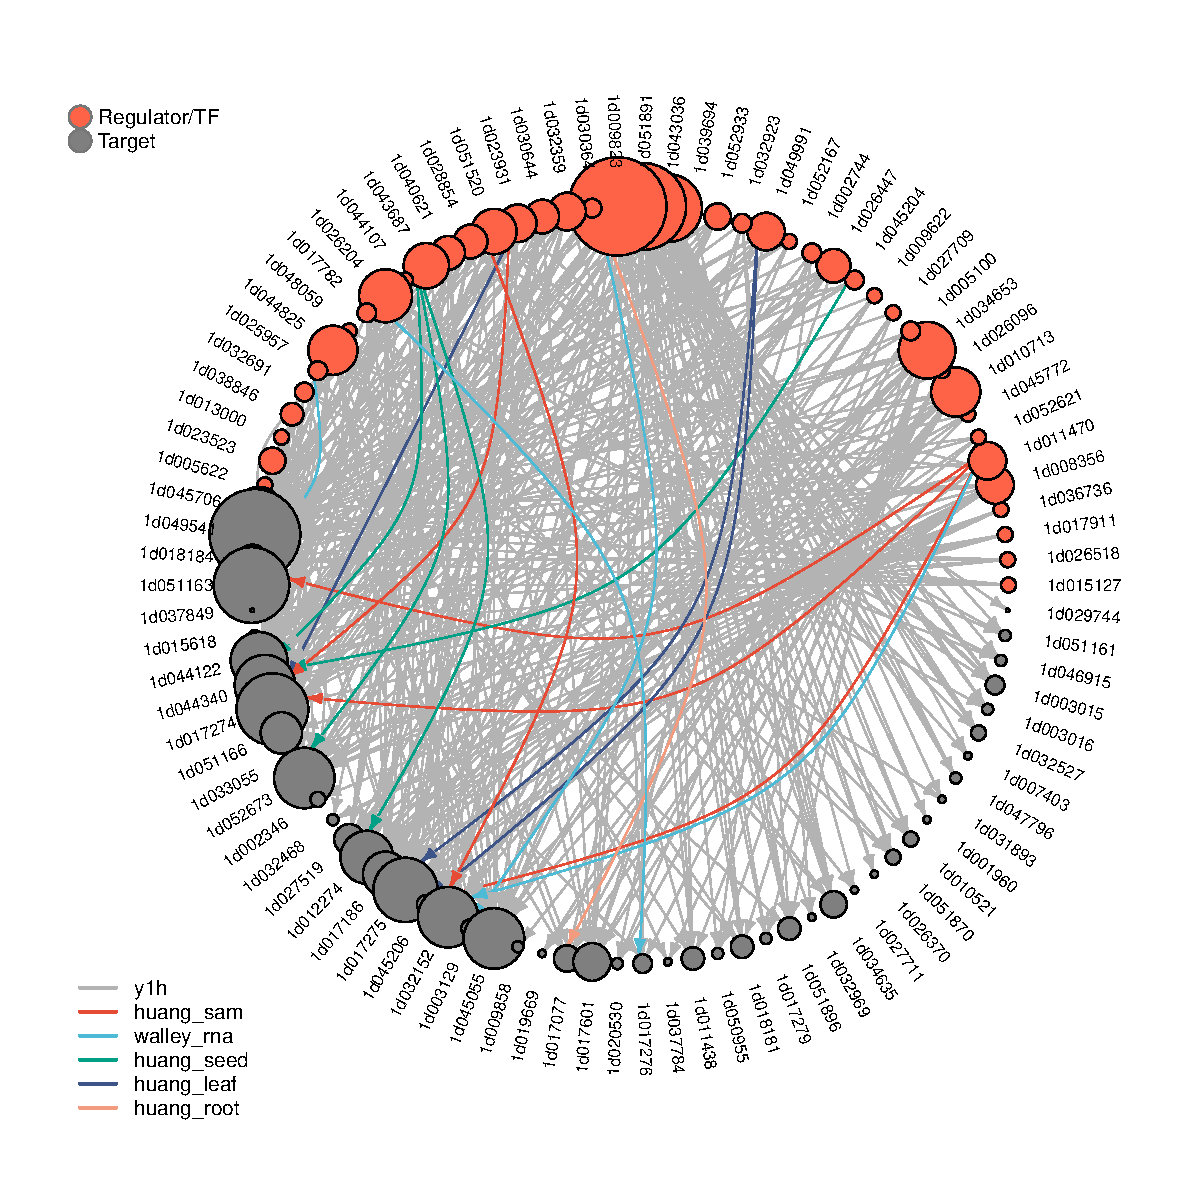
\includegraphics[width=1\textwidth,height=\textheight]{$grn/analysis/04_y1h/01.pdf}
\caption{Figure 1}
\end{figure}
\newpage
\singlespacing 
\end{document}

